%% Introduce what sequencing machines are in the context
Aligning DNA has become possible with the democratisation of \emph{sequencing machines} or \emph{sequencers}. The first sequencer was released in 1986, making it a rather recent invention. These machines take a DNA sample and find the sequences of A, T, C and G bases from it. Recent machines, belonging to what is called the \emph{third generation sequencers}, are remarkable for their long sequences reads of more than 5000 bases and their ability to compensate their low raw read precision with prediction algorithms~\cite{Lee048603}. Different techniques exists depending on the machine manufacturer. For example, one technique involves using a nanopore as an electrical sensor with a hole on which the DNA string passes, much like a sensor reading a cassette tape. The ionic composition of each base creates a different current change in the sensor, making it possible to deduce which nucleotide it is~\cite{Oxford:nanopore}.

Several questions arise from the problem of computing DNA alignment. First, we introduced the fact that the alignment should provide some kind of metric, to quantify how good the alignment is. A sample DNA is constituted of a large number of strings, all of them having the same number of bases (for example, 150 bases). This is because sequencing machines output fixed-length strings. These fixed-length strings are called \emph{query} sequences. Each of them should be aligned with a slightly longer sequence located in the reference genome. All of these sequences extracted from the genome are called the \emph{target} sequences.

As said before, these two sequences are composed of nucleotides or bases, which are reported from their first letter: A, T, C and G. We define a match score corresponding to the score when two bases are equal. In the case of DNA, mutations often take the form of adding bases, deleting bases, or changing some bases, as seen on figure~\ref{fig:mutation}. 
\begin{figure}[h!]
	\centering
	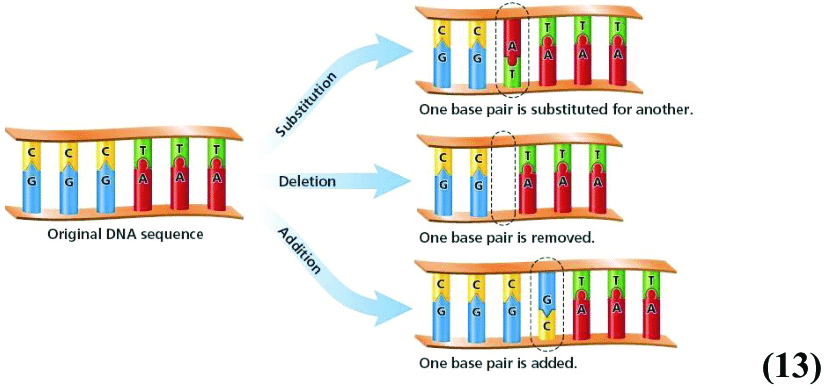
\includegraphics[width=0.7\linewidth]{mutation}
	\caption{Examples of mutation (from~\cite{alasadi:chemistry})}
	\label{fig:mutation}
\end{figure}
Mismatches can appear in the form of insertion or deletion of one or multiple bases, in either the query or the target. We then define an insertion mismatch score and a deletion mismatch score. The matching score has a positive value, and the mismatch scores are negative, and often mismatch scores are set at the same value. For the query sequences, it may happen that a base cannot be correctly retrieved by the sequencing machine, and if this happens, the unknown base is denoted as "N" and is always counted as a mismatch. Furthermore, in real-life mutations, it is much more likely to have a small number of long gaps rather than multiple short gaps. To reflect this, the model "affine gap penalty" for DNA mutation is used. We define a big mismatch score for opening a gap, and a smaller mismatch score for extending the gap. This way, during the alignment, we apply a bigger penalty when trying to open a gap rather than when a mismatch only causes a gap to get wider. 

Another challenge is to process a huge number of sequences as fast as possible. In fact, DNA sequencers produce DNA strings of a given length proper to each machine. While older sequencers produce short strings of 80 or 150 bases, more recent ones can output 7000 bases per string, and millions of strings are produced. Thanks to the fact that strings are not related to each other. There is no obstacle in processing multiple of them at the same time. This mode is called \emph{inter-sequence parallelisation}. It is also possible to parallelize the alignment calculation for each sequence, but this mode, named \emph{intra-sequence parallelisation}, requires extra care about synchronisation.

Furthermore, looking into a full genome for a match would be an incredibly tedious task without an efficient search algorithm. It is then advisable to create an index of the reference genome. With this index, operations to research a given pattern in a huge data set can be faster than linear time with respect to the data size.

